%!TEX root = ../dissertation.tex

\hypertarget{(chap:capitolo2)}{}
\chapter{Analisi dei dati}
Nel seguente capitolo vedremo com'è composto lo storico ordini e quali solo le informazioni disponibili, inoltre descriveremo con maggior dettaglio alcuni 'campi'. Inoltre verranno descritte alcune operazioni di preparazione dei dati.
\section{Principali tabelle}
Lo storico vendite dell'azienda Cliente è stato estratto dal modulo hybris, questo è organizzato secondo le tabelle SAP, avremo quindi lo storico delle fatture, composto da una tabella per la testata della fattura (VBAK), ossia la parte descrittiva dove viene riportato l'acquirente, e una tabella per le posizioni della fattura (VBAP), ossia la parte dove vengono riportati i materiali acquistati. 
Abbiamo inoltre due tabelle che contengono rispettivamente l'anagrafica cliente (KNA1) e materiali (MARA), dove possiamo trovare informazioni aggiuntive che li descrivono. 
Mi è stato inoltre fornito un glossario che riportava per ciascuna tabella una breve spiegazione di ogni campo. 
Tutte queste tabelle sono in formato Excel.
Vediamo ora per ciascuna di queste tabelle i campi annessi e alcune informazioni di natura statistica.

\subsection{Tabella VBAK}
La tabella VBAK contiene la testata di circa 35000 fatture, datate dall'anno 2016 fino a maggio 2021.\\
Ciascuna riga della tabella è la testata di una fattura e ne riporta il suo codice identificativo (\textbf{VBELN}) insieme con il codice del cliente a cui è associata (\textbf{KUNNR}). Inoltre ciascuna fattura riporta data e ora (\textbf{ERDAT}, \textbf{ERZET}) in cui è stata emessa, l'importo totale e la valuta corrispondente (\textbf{NETWR}, \textbf{WAERK}).

\subsection{Tabella VBAP}
La tabella VBAP contiene le posizioni delle fatture (circa 250000), riporta per ognuna di esse la lista di prodotti acquistati indicando diverse informazioni.
Ciascuna riga della tabella riporta quindi il codice identificativo (\textbf{VBELN}) della fattura e il codice identificativo del prodotto acquistato (\textbf{MATNR}), poi vengono riportati per quel prodotto il prezzo unitario (\textbf{NETPR}), la quantità acquistata (\textbf{KWMENG}), la spesa totale con la valuta (\textbf{NETWR}, \textbf{WAERK}) e il codice gerarchia prodotto storico (\textbf{PRODH}), ossia quello salvato in MARA al momento del'emissione della fattura.

\subsection{Tabella KNA1}
La tabella KNA1 riporta l'anagrafica cliente (circa 3000), per ciascuna riga abbiamo il codice cliente (\textbf{KUNNR}), il codice paese d'origine (\textbf{LAND1}), il nome dell'azienda (\textbf{NAME1}), la località (\textbf{ORT01}) e la regione (\textbf{REGIO}).

\subsection{Tabella MARA}
Come detto la tabella MARA è quella che riporta l'anagrafica dei materiali, nella nostra futura trattazione considereremo questi materiali come prodotti in quanto sono acquistabili all'interno dell'e-commerce.\\
Ciascuna riga della tabella riporta quindi un prodotto univoco composto dal suo usuale codice identificativo (\textbf{MATNR}), dal codice della gerarchia prodotto (\textbf{PRODH}) e del gruppo merceologico (\textbf{MATKL}) e una breve descrizione testuale (\textbf{MAKTX}), poi abbiamo delle informazioni su dimensione, volume e peso.\\
Per le dimensioni abbiamo un campo (\textbf{GROES}) che le fornisce nel formato lunghezza X larghezza X altezza, oppure altri (\textbf{LAENG}, \textbf{BREIT}, \textbf{HOEHE}), che indicano rispettivamente lunghezza, larghezza e altezza e l'unità di misura per entrambi i formati viene riportata nello stesso campo (\textbf{MEABM}). \\
Poi abbiamo due campi per volume e peso (\textbf{VOLUM}, \textbf{NTGEW}) e altri due per le loro rispettive unità di misura (\textbf{VOLEH}, \textbf{GEEWI}).

Vediamo ora nella Figura \ref{tab:sapone} il diagramma ER delle tabelle sopra descritte con le relative dipendenze.
\begin{center}
	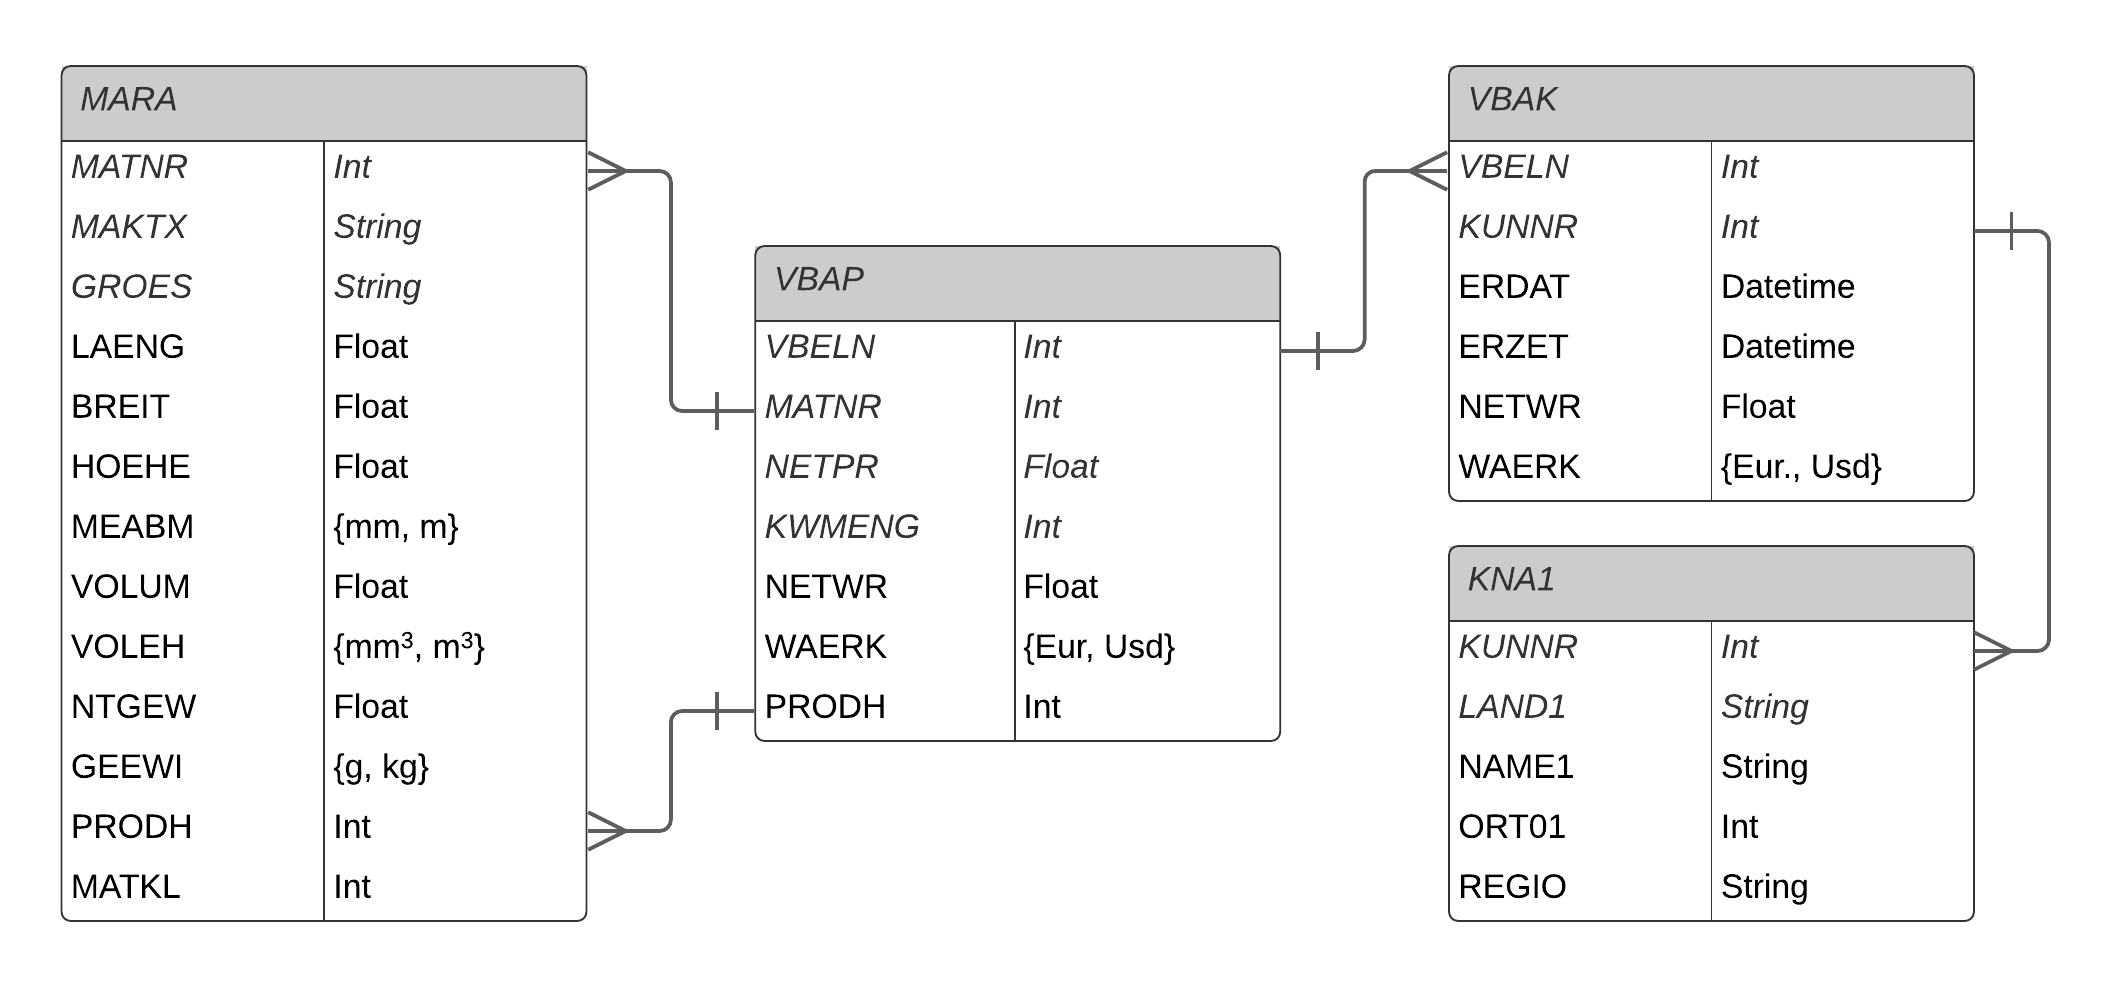
\includegraphics[width=13cm]{figures/ER_sap.png}
	\captionof{figure}{Diagramma ER tabelle Mara, Kna1, Vbak e Vbap.}
	\label{tab:sapone}
\end{center}

\section{Prodotti}
Da questo momento in poi faremo riferimento ai materiali chiamandoli prodotti come detto in precedenza.\\
In totale nella tabella anagrafica materiali (MARA) sono presenti circa 75000 prodotti diversi, mentre i prodotti effettivamente venduti risultano essere molti meno attestandosi all'incirca verso gli 8000.\\
Abbiamo però due campi interessanti che riguardano la gerarchia prodotto (PRODH) e il gruppo merceologico (MATKL), questi due ci permettono di studiare la similarità dei prodotti.

\subsection{Gerarchia prodotto (PRODH)}
Il campo gerarchia prodotto (PRODH) è un campo numerico di 18 cifre utile per separare i prodotti rispetto le diverse categorie su più livelli.
Nella tabella secondaria T179 vengono definiti i livelli di gerarchia e le diverse categorie, abbiamo il codice gerarchia prodotto (\textbf{PRODH}), il livello (\textbf{STUFE}) e il titolo (\textbf{VTEXT}), quindi la tabella Mara fa riferimento a questa come mostrato nella Figura \ref{tab:er_t179}.
\begin{center}
	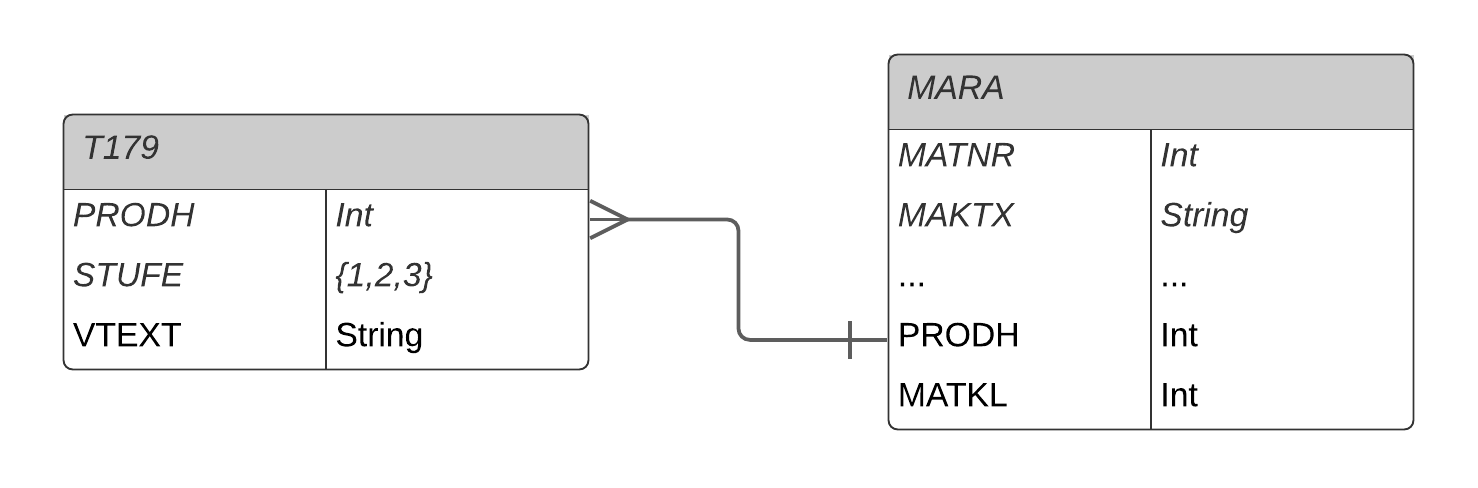
\includegraphics[width=10cm]{figures/ER_T179.png}
	\captionof{figure}{Diagramma ER tabelle Mara e T179.}
	\label{tab:er_t179}
\end{center}

Ciascun codice PRODH contenuto nella tabella T179 avrà rispettivamente il seguente numero di cifre in base al livello di gerarchia (STUFE):
\begin{itemize}
	\item \textbf{STUFE = 1}: 1° livello della gerarchia, il codice sarà di 5 cifre;
	\item \textbf{STUFE = 2}: 2° livello della gerarchia, il codice sarà di 10 cifre, dove le prime 5 identificano la categoria di 1° livello a cui appartengono mentre le restanti 5 indentificano la sotto-categoria di 2° livello;
	\item \textbf{STUFE = 3}: 3° livello della gerarchia, il codice sarà di 18 cifre, dove le prime 10 identificano la categoria di 2° livello a cui appartengono mentre le restanti 8 indentificano la sotto-categoria di 3° livello.
\end{itemize}
Ciascun prodotto sarà quindi provvisto di un codice di 18 cifre che identificherà una categoria per ogni livello.\\
Nella tabella VBAP ci sono alcune posizioni dove a parità di codice prodotto (MATNR) si hanno codici PRODH diversi, questo è dovuto al diverso momento temporale in cui sono stati acquistati, infatti nella tabella VBAP il codice PRODH è storico, ho provveduto per semplicità ad aggiornarli tutti al codice PRODH più recente riportato nella tabella anagrafica materiali MARA.
Il numero di prodotti interessati sono circa 100 su 10000 posizioni.\\
\subsubsection{Selezione categorie di 1° livello}

\begin{minipage}[H]{0.50\textwidth}
	\begin{center}
	\scalebox{0.55}{%
	\begin{tabular}{|l|rr|l|}
		\toprule
		PRODH &    $\#tot$ &  $\#sold$ &                  titolo \\
		\midrule
		00010 &    28 &    0 &              categoria1 \\ %               Lavasciuga \\
		00020 &     0 &    0 &              categoria2 \\ %              Spazzatrici \\
		00030 &     0 &    0 &              categoria3 \\ %             Monospazzole \\
		00040 &     5 &    0 &              categoria4 \\ %               Aspiratori \\
		00050 &     2 &    0 &              categoria5 \\ %      Car washing system \\
		00090 &     2 &    0 &              categoria6 \\ %      Ricambi / accessori \\
		00100 &  1117 &  173 &              CATEGORIA1 \\ %  LAVASCIUGA UOMO A TERRA \\
		00200 &   645 &  130 &              CATEGORIA2 \\ %  LAVASCIUGA UOMO A BORDO \\
		00250 &    31 &   11 &              CATEGORIA3 \\ %             SANIFICATORI \\
		00300 &   405 &   92 &              CATEGORIA4 \\ %              SPAZZATRICI \\
		00400 &   525 &   36 &              CATEGORIA5 \\ %             MONOSPAZZOLE \\
		00500 &  1715 &   70 &              CATEGORIA6 \\ %               ASPIRATORI \\
		00600 &   334 &    6 &              CATEGORIA7 \\ %           WASHING SYSTEM \\
		00700 &     1 &    0 &              CATEGORIA8 \\ %          SISTEMI RICICLO \\
		00900 & 70441 & 7702 &              CATEGORIA9 \\ %      RICAMBI \& ACCESSORI \
		00950 &    28 &    1 &             CATEGORIA10 \\ %                CHEMICALS \\
		09999 &   215 &    0 &                   ALTRO \\ %                    ALTRO \\
		\bottomrule
	\end{tabular}
}
\captionof{table}{Categorie (PRODH) 1°\\ livello, unità totali e vendute.}
\label{tab:PRODH_tot}
\end{center}

\end{minipage}
\begin{minipage}[H]{0.50\textwidth}
Nella tabella \ref{tab:PRODH_tot} vengono mostrati i codici PRODH delle categorie di 1° livello, nella colonna $\#tot$ il numero di prodotti diversi per quella categoria, nella colonna $\#sold$ il numero di prodotti diversi acquistati almeno una volta appartententi a quella categoria ed infine il titolo della categoria.\\
Come possiamo vedere le prime sei categorie con titolo in minuscolo hanno pochi prodotti catalogati in MARA e nessun prodotto venduto.\\
\end{minipage}\\

Chiaramente il fatto che siano tutti a zero è dovuto all'aggiornamento dei codici PRODH di cui abbiamo parlato precedentemente, a prescindere da ciò il numero di posizioni che prima riportavano codici appartenenti alle categorie prese in considerazione non superava la decina, quindi non considerare queste categorie in quanto si è smesso di usarle sembra la scelta più logica.\\
La categoria ALTRO (09999) non è stata considerata in quanto riporta prodotti che non sono disponibili sull'e-commerce.
Inoltre le categorie CATEGORIA8 (00700) e CATEGORIA10 (00950), dato il basso numero di prodotti presenti in MARA e le basse vendite, si è preferito non considerarle.
\subsubsection{Overview categorie di 1° livello}
\begin{center}
\scalebox{0.6}{%
\begin{tabular}{|l|rrrccc|l|}
\toprule
$PRODH$ &    $\#posizioni$ &  $\sum_{KWMENG}$ &  $\mathbb{E}_{KWMENG}$ &     $\mathbb{E}_{NETPR}$ &     $\sum_{NETWR}$ &     $\mathbb{E}_{NETWR}$ &      $titolo$\\
      &                  &              &              &       (€)      &      (€)       &        (€)     &            \\
\midrule
00100 &      5908 &    15461 &    2.61 &   1613.44 &   3865.97 &  22840167.61 &  CATEGORIA1 \\
00200 &      1936 &     3219 &    1.66 &   5898.09 &   8640.59 &  16745496.87 &  CATEGORIA2 \\
00250 &       333 &     2949 &    8.85 &    552.99 &   3772.04 &   1377422.72 &  CATEGORIA3 \\
00300 &       745 &     1390 &    1.86 &   4353.24 &   5364.34 &   3996430.94 &  CATEGORIA4 \\
00400 &       389 &     1651 &    4.24 &    708.17 &   2404.47 &    940777.84 &  CATEGORIA5 \\
00500 &      1133 &    12984 &   11.46 &    175.75 &   1034.63 &   1172236.58 &  CATEGORIA6 \\
00600 &       153 &      494 &    3.23 &    448.52 &   1338.80 &     83501.04 &  CATEGORIA7 \\
00900 &    239740 &  1070334 &    4.46 &     26.67 &     66.61 &  15968039.56 &  CATEGORIA9 \\
\midrule
      &   250339  &  1108493.51 &   4.72 & 1706.86 &   3225.75 &  63124073.16 &       valori riassuntivi \\

\bottomrule
\end{tabular}}
\captionof{table}{Informazioni sulle categorie (PRODH) 1° livello selezionate}
\label{tab:PRODH_sel}
\end{center}

Nella tabella \ref{tab:PRODH_sel} per ogni categoria $PRODH$ di 1° livello possiamo vedere:
\begin{itemize}
	\item $\#posizioni$: numero di posizioni in cui compaiono prodotti di quella categoria in fattura;
	\item $\sum_{KWMENG}$: quantità totale di prodotti acquistati appartenenti a quella categoria;
	\item $\mathbb{E}_{KWMENG}$: quantità media per fattura di prodotti acquistati appartenti a quella categoria;
	\item $\mathbb{E}_{NETPR}$: prezzo medio per fattura di prodotti acquistati di quella categoria;
	\item $\sum_{NETWR}$: spesa totale per prodotti di quella categoria;
	\item $\mathbb{E}_{NETWR}$: spesa totale media per fattura di prodotti di quella categoria.
\end{itemize}
Dalla tabella possiamo vedere come la categoria RICAMBI \& ACCESSORI riporti un prezzo medio per fattura molto più basso rispetto alle altre categorie, questo è dovuto al fatto che i pezzi di ricambio ed accessori non sono macchine o sistemi da usare per fornire un servizio quanto un prodotto per riparare ciò che già si possiede. Possiamo vedere che in termini di posizioni l'acquisto di pezzi di ricambio copra una cospicua parte delle posizioni in fattura, oltre che costituire un'importante parte del fatturato per l'azienda. Le altre categorie indicano macchine e sistemi per la pulizia quindi il prezzo medio per prodotto è molto maggiori e per i clienti finali questi rappresentano un investimento.\\
Da quanto detto finora si vengono a creare due macro categorie di prodotti:
\begin{itemize}
	\item \textbf{Macchine}: questa macro categoria racchiude sette categorie di 1° livello (00100, 00200, 00250, 00300, 00400, 00500, 00600);
	\item \textbf{Ricambi}: questa macro categoria invece racchiude la sola categoria 00900.
\end{itemize}

Dobbiamo dare un'ultima precisazione, la maggior parte delle categorie di 2° e 3° livello risultano essere di prodotti appartenenti alla macro categoria delle macchine, quindi la gerarchia è molto più densa orizzontalmente per le macchine rispetto che i pezzi di ricambio, infatti per le macchine le categorie risultano essere i diversi modelli di macchinari disponibili e i prodotti a catalogo di quella categoria sono le varianti dello stesso modello di macchinario. Per i pezzi di ricambio abbiamo solo poche categorie contenitore che li raggruppano tutti insieme.

\subsection{Gruppo merceologico (MATKL)}
Il gruppo merceologico (MATKL) non è organizzato come una gerarchia, come lo è invece la gerarchia prodotto (PRODH), bensì come un insieme di prodotti, in totale abbiamo circa 160 gruppi, dove uno di questi contiene tutti i prodotti che prima abbiamo classificato come macchine. Rispetto il codice PRODH, il gruppo merceologico è più divisivo rispetto i ricambi, questo ci può aiutare in quanto ora siamo in grado di categorizzare anche i ricambi. 

\subsection{Dimensione, volume e peso}
I campi rigurdanti dimensione, volume e peso potrebbero essere utili per ricercare una similarità tra i prodotti.\\
Le informazioni sulle dimensioni, come lunghezza, larghezza e altezza sono praticamente ridondanti nei campi GROES e (LAENG, BREIT, HOEHE) se non per alcuni prodotti dove le informazioni sono esclusive di uno dei due formati.\\
Per peso e volume abbiamo i rispettivi campi numerici e altri due campi che riportano le unità di misura, per il volume possono essere i metri cubi o i millimetri cubi, per il peso i kilogrammi o i grammi.
La criticità di queste misure riguarda la loro scarsità, infatti su 75000 prodotti abbiamo informazioni su volume e peso rispettivamente solo sul 20\% e 39\%, mentre sui prodotti acquistati almeno una volta sul 19\% e 5\%. 

\subsection{Preprocessing dati}
In questa sezione andremo a vedere quali operazioni si sono rese necessarie per preparare i dati:
\begin{itemize}
	\item posizioni con spesa totale nulla sono stati eliminati;
	\item posizioni con valuta in $Usd$ sono state convertiti in $Eur$;
	\item prodotti con misure di dimensione e volume, con unità di misura diversa rispettivamente dai $metri$ e $metri^3$, sono stati convertiti negli stessi;
	\item prodotti con misure del peso con unità di misura diverse dal $kilogrammo$ sono state convertite nello stesso;
	\item alcuni clienti non sono stati considerati in quanto appartenenti allo stesso gruppo dell'azienda Cliente.
\end{itemize}